\chapter{Fundamentação teórica}

Este capitulo apresentada conceitos, técnicas e ferramentas relevantes ao desenvolvimento
do trabalho e à compreensão das próximas seções. O capítulo abrange fundamentos sobre arquitetura de \textit{software}, banco de dados e processo de desenvolvimento de \textit{software}.

\section{Arquitetura de \textit{software}}
\label{fundArquietura}

Sistemas grandes são sempre decompostos em subsistemas que fornecem algum conjunto de serviços relacionados. O processo inicial de projeto, que consiste em identificar esses subsistemas e estabelecer um \textit{framework} para o controle e a comunicação de subsistemas, é denominado projeto de arquitetura de software. \cite{sommerville}

A arquitetura de software; portanto, refere-se aos componentes de alto nível de um sistema de \textit{software} e à disciplina de criação destes. Cada um dos seus componentes incorpora elementos de \textit{software}, suas inter-relações e propriedades que os constituem. Além disso, define tarefas necessárias para serem realizadas pelas equipes que constituem o projeto.


\subsection{Arquitetura cliente-servidor}
\label{arquiteturaCentralizadaDados}

O modelo de arquitetura cliente-servidor é é um modelo em que o sistema é organizado como um conjunto de serviços e servidores e clientes associados acessam e usam estes serviços. Os clientes geralmente precisam saber nome e serviços disponíveis que os servidores oferecem. No entanto, servidores não precisam saber nomes nem quantos clientes existem. Essencialmente, um cliente faz um pedido a um servidor e espera até receber uma resposta. \cite{pressman}. Exemplos de aplicativos de computador que usam o modelo cliente-servidor são \textit{e-mail}, impressão em rede e a Internet.


\subsection{Arquitetura centrada em dados}
\label{arquiteturaCentralizadaDados}

Arquitetura centrada em dados é um modelo de arquitetura de \textit{software} onde os bancos de dados são imprescindíveis para o funcionamento do sistema. Um sistema provido desta arquitetura processa solicitações de usuários a um banco de dados ou solicitações para atualizar o banco de dados \cite{lewisBook}. A Figura \ref{dataCenteredArchitecture} exibe um estilo típico de arquitetura centrada em dados.

\begin{figure}[ht]
    \caption{Arquitetura centrada em dados.}
       	\begin{center}
            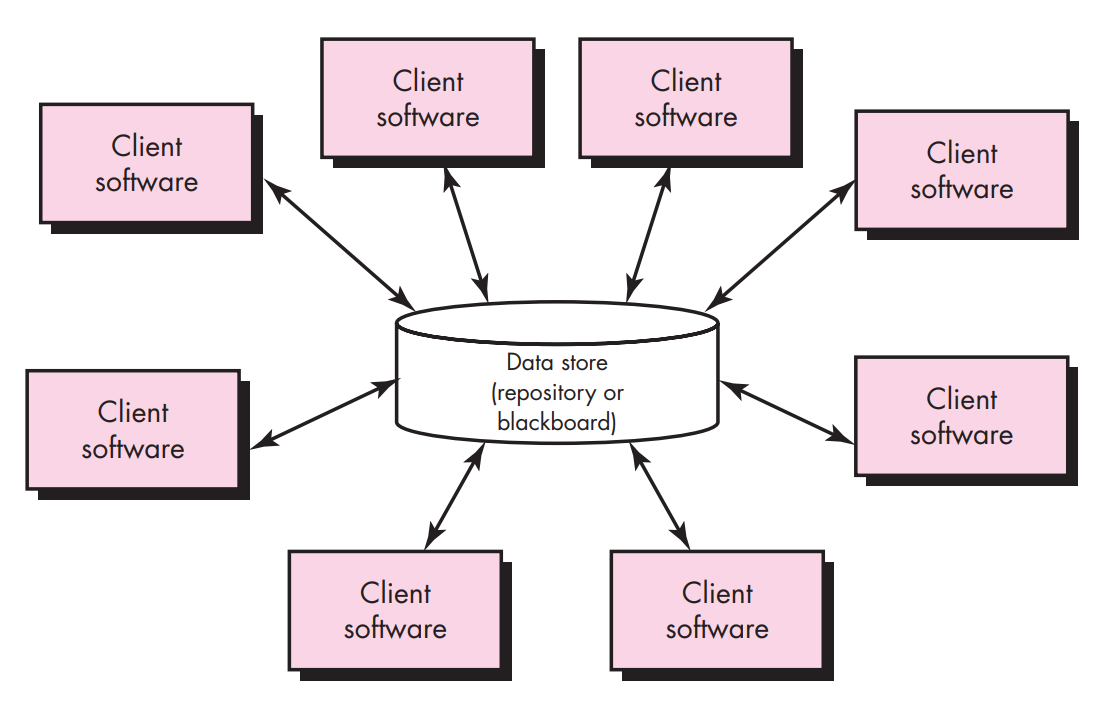
\includegraphics[width=0.75\textwidth]{arquitetura-centralizada-dados.png}
        \end{center}
    \label{dataCenteredArchitecture}
    \legend{
        \textit{Software} cliente acessa um repositório central independentemente de quaisquer alterações nos dados ou ações de outro \textit{software} cliente. \cite{pressman}
    }
\end{figure}


\subsection{Arquitetura MVC}
\label{arquiteturaMVC}

A arquitetura MVC, Modelo-visão-controlador, é um padrão arquitetural comumente usado para desenvolver interfaces de usuário que divide um aplicativo em três partes interconectadas: modelo, visão e controlador \cite{mvcCookbook}. Este padrão de arquitetura desacopla os três componentes principais, permitindo a reuso mais eficiente de código e desenvolvimento paralelo entre eles. 

O modelo engloba todo domínio específico à aplicação e seu processamento lógico como funcionalidades e acesso a dados externos e fontes de informação. A visão é responsável por exibir, na saída de dados, o conteúdo do modelo em um formato legível e requisitado pelo usuário final. O controlador coordena a comunicação entre o modelo e a visão de acordo com as requisições do usuário. A Figura \ref{dataMVCArchitecture} ilustra a arquitetura MVC.

\begin{figure}[ht]
    \caption{Arquitetura MVC em aplicação \textit{web}.}
       	\begin{center}
            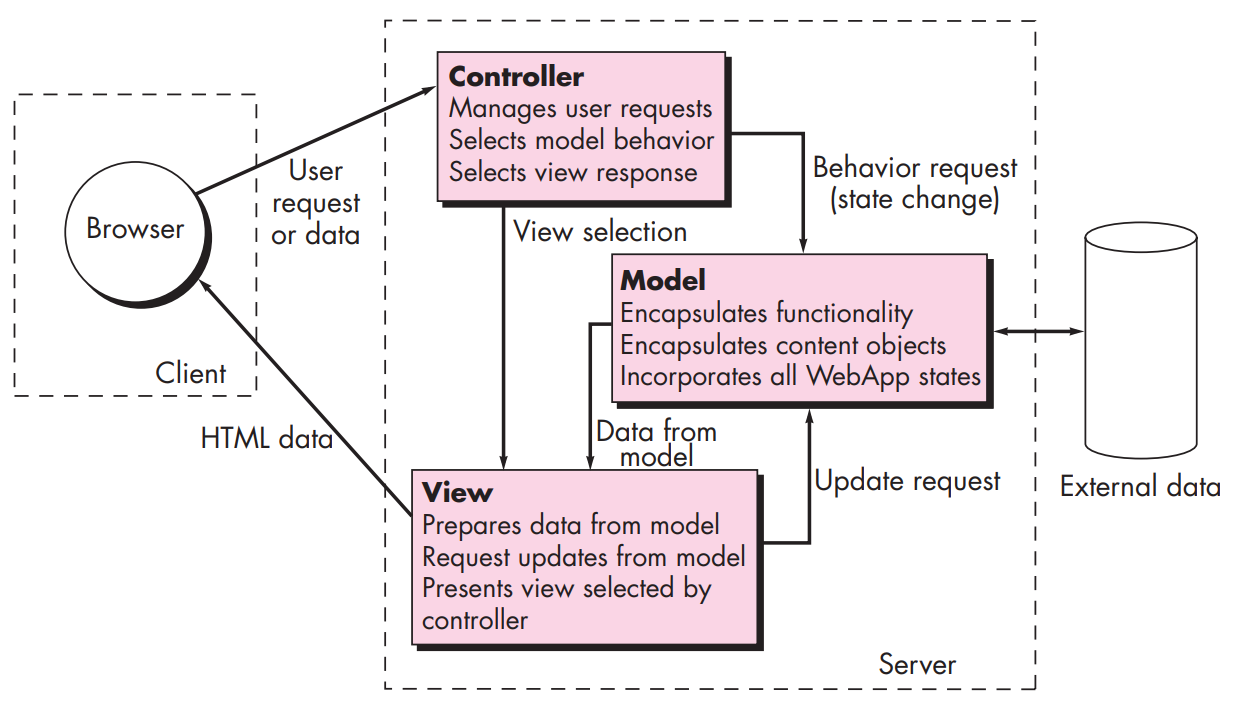
\includegraphics[width=0.75\textwidth]{arquitetura-mvc.png}
        \end{center}
    \label{dataMVCArchitecture}
    \legend{Fonte: \cite{pressman}}
\end{figure}


\section{Banco de dados}
\label{fundBD}

Um banco de dados pode ser definido como um conjunto de dados integrados que tem por objetivo atender a uma comunidade de usuários \cite{heuser}. Eles possuem uma coleção organizada de dados, geralmente armazenados e acessados por \textit{softwares} de computador. Devido aos avanços tecnológicos nessa área, bancos de dados foram aumentando sua complexidade e, para manter um sistema robusto, que incorpora funções de definição, alteração e recuperação, são utilizados SGBDs.

Contudo, o processo de criação de um banco de dados para o \textit{software} de uma aplicação sugere a utilização de técnicas de construção de um projeto de banco de dados. No projeto, são considerados dois níveis de abstração de modelo de dados para sua implementação: o modelo conceitual e o modelo lógico.

\subsection{Modelo conceitual}
\label{fundBDModelagem}

A modelagem conceitual é utilizada para obter uma descrição abstrata, independente de implementação em computador, dos dados que serão armazenados no banco de dados. A técnica de modelagem de dados mais difundida e utilizada é a abordagem entidade-relacionamento (ER). \cite{heuser} Através dela, os modelos de dados são representados graficamente por um diagrama entidade-relacionamento (DER). A figura \ref{modelagemBDExemplol} apresenta um DER parcial presente na modelagem conceitual do sistema implementado.

\begin{figure}[h]
    \caption{Exemplo de modelagem conceitual.}
       	\begin{center}
            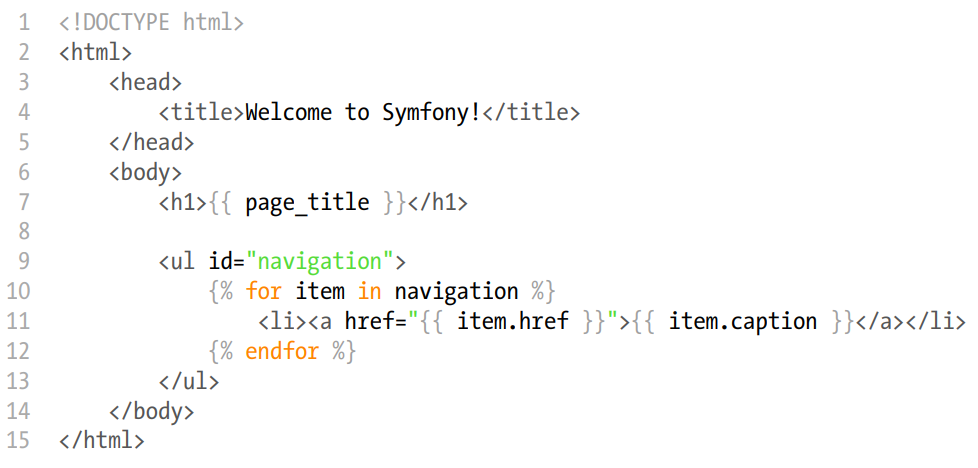
\includegraphics[width=0.68\textwidth]{figuras/twig-symf.png}
        \end{center}
    \label{modelagemBDExemplol}
    \legend{Fonte: Autor}
\end{figure}

\subsection{Modelo lógico}
\label{fundBDProjeto}

O projeto lógico consiste na transformação de um modelo ER em um modelo lógico. Este implementa de forma concreta, a nível de SGBD relacional, os dados representados no modelo ER.

Um determinado modelo ER pode ser implementado através de diversos modelos relacionais, que contém as informações especificadas pelo diagrama ER. Todos podem ser considerados uma implementação correta do modelo ER considerado. Entretanto, diferentes modelos relacionais podem resultar em diferentes performances do sistema construído sobre o banco de dados. 

No processo de transformação do modelo ER para o modelo relacional, foram utilizadas as seguintes regras de transformação \cite{heuser} a fim de obter uma melhor performance do sistema: 

\begin{itemize}
    \item Obter um banco de dados que permita boa performance de instruções de consulta e alteração do banco de dados.
    
    \item Obter um banco de dados que simplifique o desenvolvimento e a manutenção de aplicações.
    
    \item Evitar junções, ou seja, ter os dados necessários a uma consulta em uma única linha.
    
    \item Diminuir o número de chaves primárias.
    
    \item Evitar campos opcionais.
    
\end{itemize}

A Figura \ref{modelagemBDLogicoExemplol} apresenta a transformação do modelo ER para o modelo relacional do exemplo apresentado na figura \ref{modelagemBDExemplol}.

\begin{figure}[h]
    \caption{Exemplo de modelagem relacional.}
       	\begin{center}
            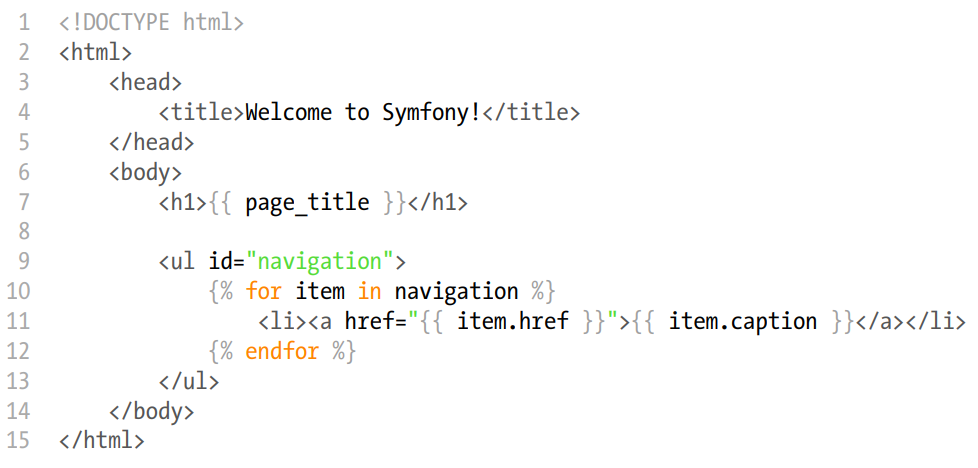
\includegraphics[width=0.68\textwidth]{figuras/twig-symf.png}
        \end{center}
    \label{modelagemBDLogicoExemplol}
    \legend{Fonte: Autor}
\end{figure}


\section{Processo de desenvolvimento de \textit{software}}

asudhia

\subsection{Metologia ágil}
\label{fundSWAgil}

a

\subsection{SCRUM}
\label{fundSWSCRUM}

b